\section{Experimental Methodology}
\label{sec:method}

In the methodology we answer the following questions:
\begin{itemize}
	\item{What workloads did we choose to run for our experiments and why?}
	\item{Are Spark and Giraph in need of more Java Heap or more cache for IO?}
	%\item{What kind of metrics should someone use to be accurate when measuring performance?}
	\item{Is cost a contributing factor to pursuing higher throughput for a server?}
\end{itemize}

\subsection{Workloads}
For our experiments, we selected four specific workloads from two
different categories of the Spark Bench suite \cite{Spark-Bench}: Page Rank (PR) and Connected
Component (CC) from GraphX and Linear Regression (LinR) and Logistic Regression (LogR)
from MLLib. For Giraph we choose PageRank, Weakly Connected Component and Community detection 
using label propagation (CDLP) from LDBC Graphalytics \cite{ldbc}. The primary reason for selecting these workloads for Spark is that
they represent different types of algorithms: PR, CC 
and are graph-based workloads, while LinR and LogR are machine learning
workloads. Giraph is a graph processing framework so we used only graph workloads. Furthermore, all of them are
well-established workloads that are commonly used for benchmarking big
data analytics systems, making them a suitable choice for our
experiments. Overall, the selection of these workloads allows us to
evaluate the performance of TeraHeap in a variety of contexts and
provide insights into the effectiveness of such an approach for improving
server throughput in managed big data analytics systems.

\subsubsection{PageRank}
PageRank is a widely used graph-based algorithm that measures the
importance of nodes in a network. It has become a popular benchmark
for evaluating the performance of distributed systems, including big
data analytics systems like Apache Spark. PageRank is computationally
intensive and requires significant memory and I/O resources, making it
a suitable workload for evaluating the performance of our TeraHeap
for improving server throughput. Additionally, PageRank is a
common algorithm in real-world applications, such as search engines
and social networks, making it relevant for practical use cases.

\subsubsection{LinearRegression}
LinearRegression is a machine learning algorithm that is used to
predict numerical values based on input data. It is a well-known and
widely used algorithm in machine learning, and is commonly used for
regression analysis in fields such as economics, finance, and
engineering. LinearRegression is computationally intensive and
requires significant memory and I/O resources, making it a suitable
workload for evaluating the performance of TeraHeap for
improving server throughput. Furthermore, the inclusion of a machine
learning workload like LinearRegression allows us to investigate the
performance of TeraHeap across different types of big data
analytics tasks and gain insights into the effectiveness of TeraHeap
for improving server throughput in a range of contexts.

\subsubsection{Logistic Regression}
LogisticRegression is a machine learning algorithm that is used to
model the probability of a binary or categorical outcome based on one
or more independent variables. It is commonly used in predictive
analytics to classify data based on historical data. In Spark-bench,
LogisticRegression is implemented as a machine learning workload,
where the dataset is represented as an RDD of feature vectors and
labels. The LogisticRegression workload involves training a logistic
regression model on the dataset, using an iterative optimization
algorithm such as gradient descent. The workload is computationally
intensive and requires a significant amount of memory to store the
dataset and model parameters.

\subsubsection{Connected Component}
ConnectedComponent is a graph algorithm that is used to identify the
connected components of a graph. It is commonly used in social network
analysis to identify clusters of users with similar interests or
relationships. In Spark-bench, ConnectedComponent is implemented as a
graph processing workload, where the graph is represented as an RDD of
edges and vertices. The ConnectedComponent workload involves iterating
over the graph, identifying the connected components of each node, and
merging the components as necessary. The workload is computationally
intensive and requires a significant amount of memory to store the
graph.

\subsubsection{Weakly Connected Component}
empty

\subsubsection{Community Detection Label Propagation}
empty

\subsubsection{}
\begin{figure}[thbp]
	\centering
    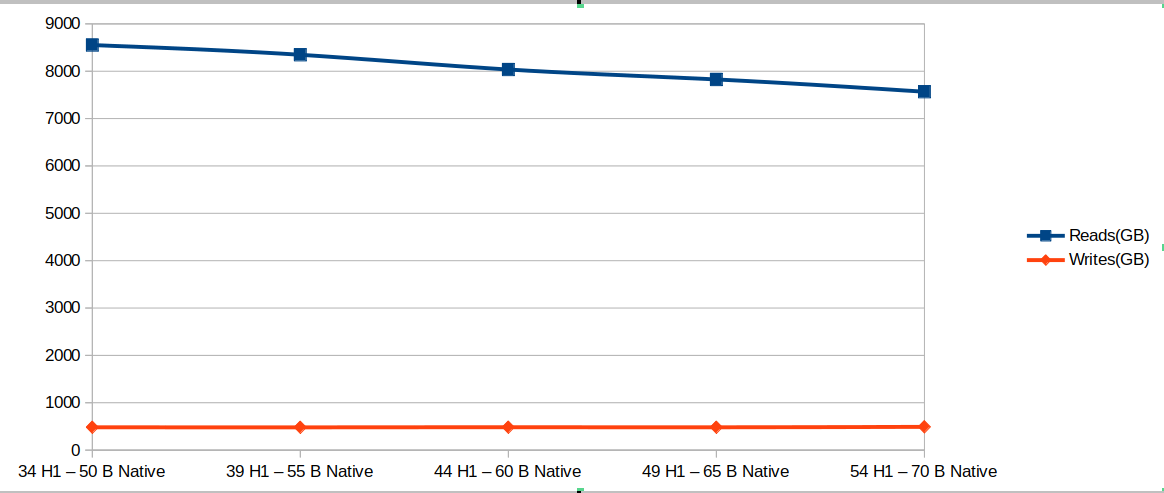
\includegraphics[width=\linewidth]{./fig/gcs_linr_h1_native.png}
    \caption{Number of GCs over time for H1 Linear Regression Native
    Spark investigation.}
    \label{fig:gcs_linr_h1_native}

    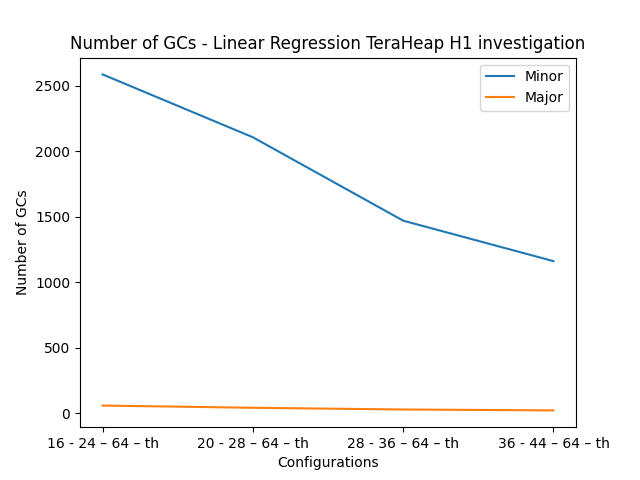
\includegraphics[width=\linewidth]{./fig/gcs_linr_h1_th.png}
    \caption{Number of GCs over time for H1 Linear Regression TeraHeap
    Spark investigation.}
    \label{fig:gcs_linr_h1_th}
\end{figure}

\begin{figure}[thbp]
    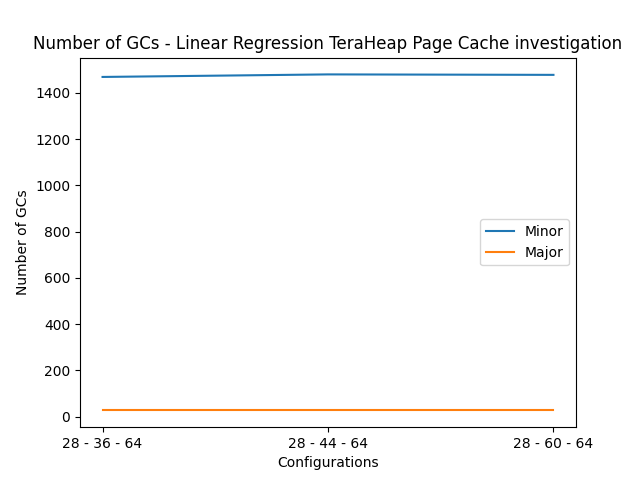
\includegraphics[width=\linewidth]{./fig/gcs_linr_pc_th.png}
    \caption{Number of GCs over time for Page Cache Linear Regression
    TeraHeap Spark investigation.}
    \label{fig:gcs_linr_pc_th}  

    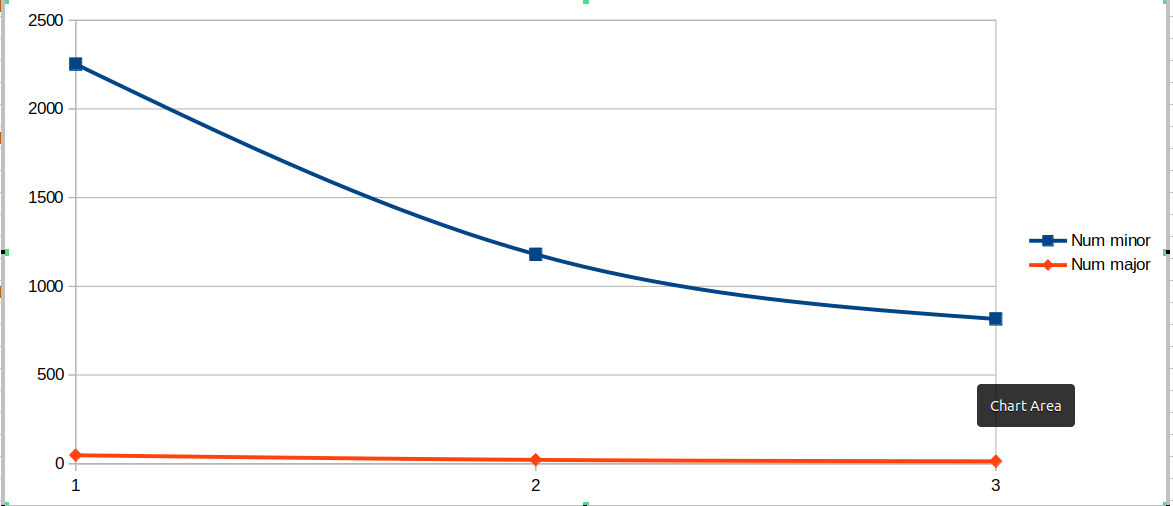
\includegraphics[width=\linewidth]{./fig/gcs_pr_h1_th.png}
    \caption{Number of GCs over time for H1 Page Rank TeraHeap Spark
    investigation.}
    \label{fig:gcs_pr_h1_th}
\end{figure}

\begin{figure}[thbp]
    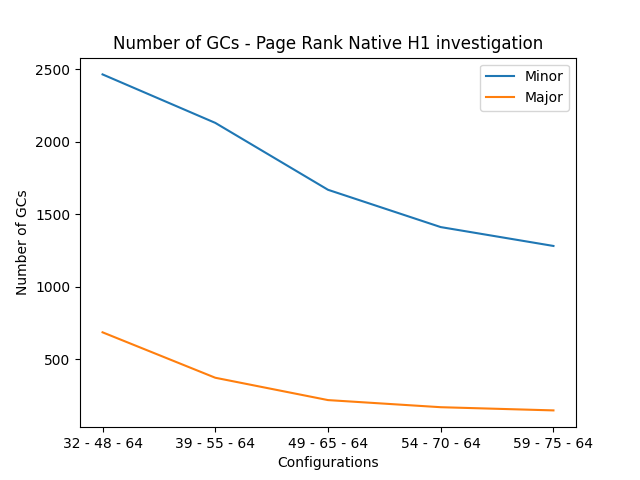
\includegraphics[width=\linewidth]{./fig/gcs_pr_h1_native.png}
    \caption{Execution time breakdown for H1 Linear Regression Native
    Spark investigation.}
    \label{fig:gcs_pr_h1_native}

    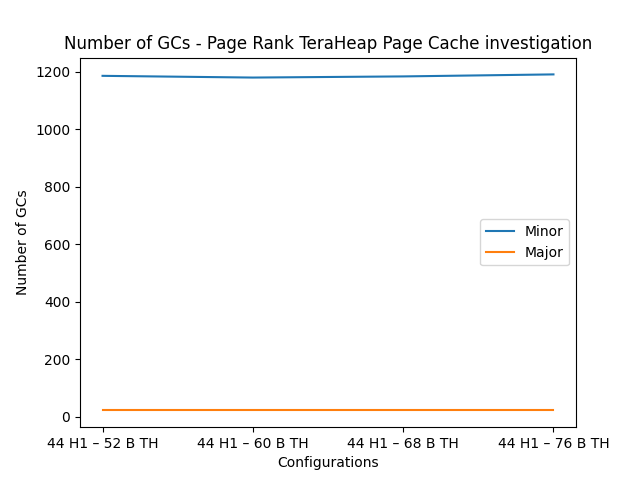
\includegraphics[width=\linewidth]{./fig/gcs_pr_pc_th.png}
    \caption{Execution time breakdown for PageCache Page Rank TeraHeap
    Spark investigation.}
    \label{fig:gcs_pr_pc_th}
\end{figure}

\begin{figure}[thbp]
    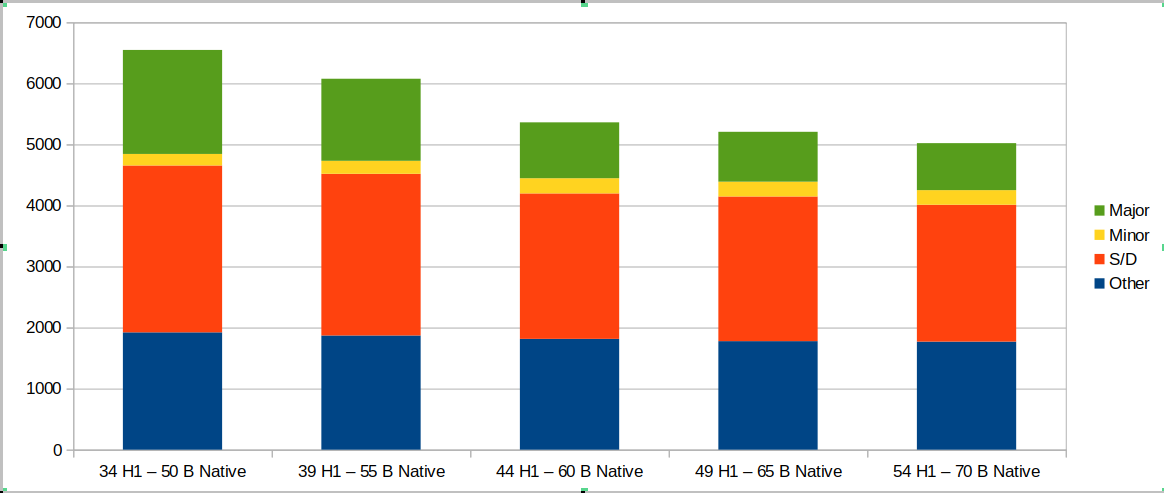
\includegraphics[width=\linewidth]{./fig/linr_h1_native.png}
    \caption{Execution time breakdown for H1 Linear Regression Native
    Spark investigation.}
    \label{fig:linr_h1_native}

    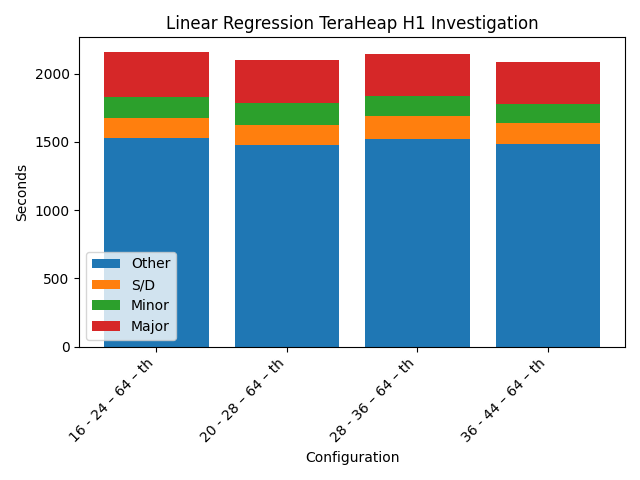
\includegraphics[width=\linewidth]{./fig/linr_h1_th.png}
    \caption{Execution time breakdown for H1 Linear Regression
    TeraHeap Spark investigation.}
    \label{fig:linr_h1_th}
\end{figure}

\begin{figure}[thbp]
    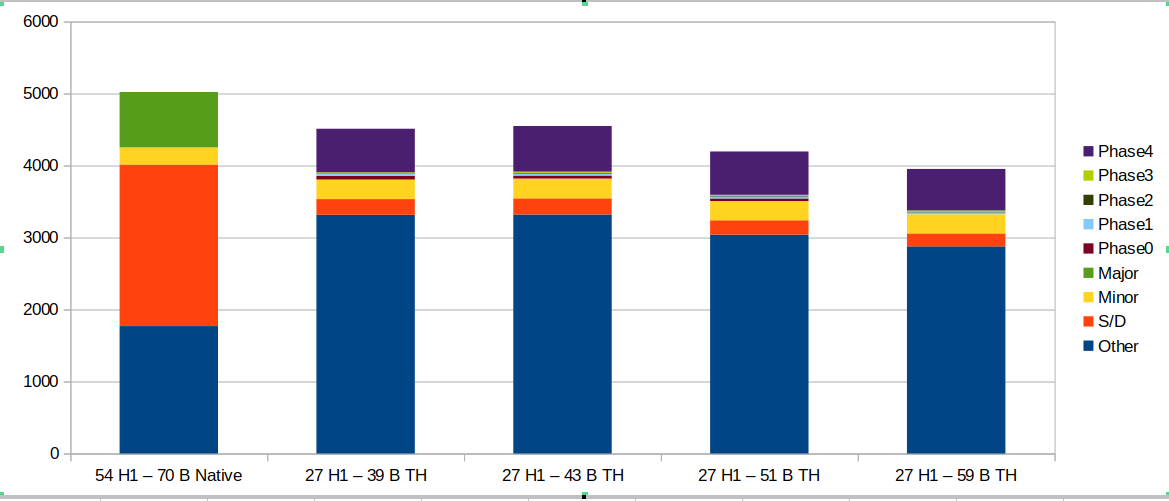
\includegraphics[width=\linewidth]{./fig/linr_pc_th.png}
    \caption{Execution time breakdown for Page Cache Linear Regression TeraHeap Spark investigation.}
    \label{fig:linr_pc_th}

    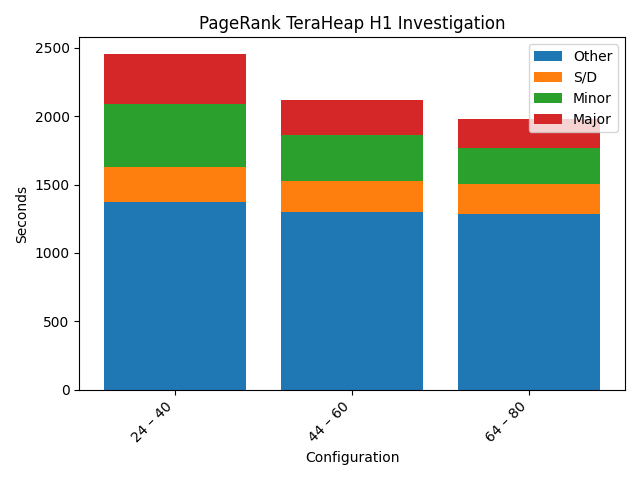
\includegraphics[width=\linewidth]{./fig/pr_h1_th.png}
    \caption{Execution time breakdown for H1 Page Rank TeraHeap Spark
    investigation.} 
    \label{fig:pr_h1_th}
\end{figure}

\begin{figure}[thbp]
    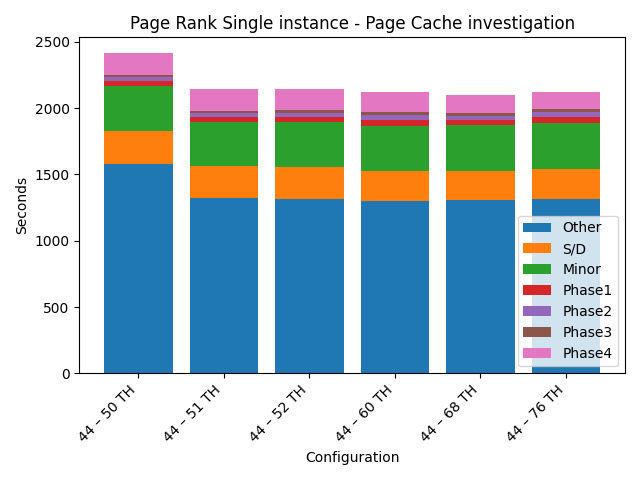
\includegraphics[width=\linewidth]{./fig/pr_pc_th.png}
    \caption{Execution time breakdown for PageCache Page Rank TeraHeap
    Spark investigation.}
    \label{fig:pr_pc_th}

    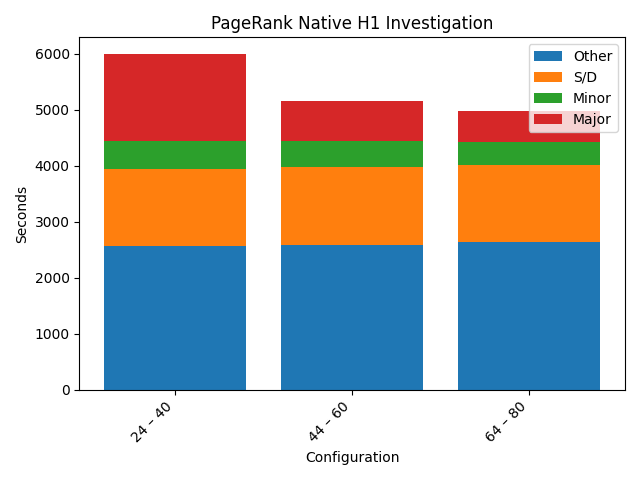
\includegraphics[width=\linewidth]{./fig/pr_h1_native.png}
    \caption{Execution time breakdown for PageCache Page Rank TeraHeap
    Spark investigation.}
    \label{fig:pr_h1_native}
\end{figure}

\begin{figure}[thbp]
    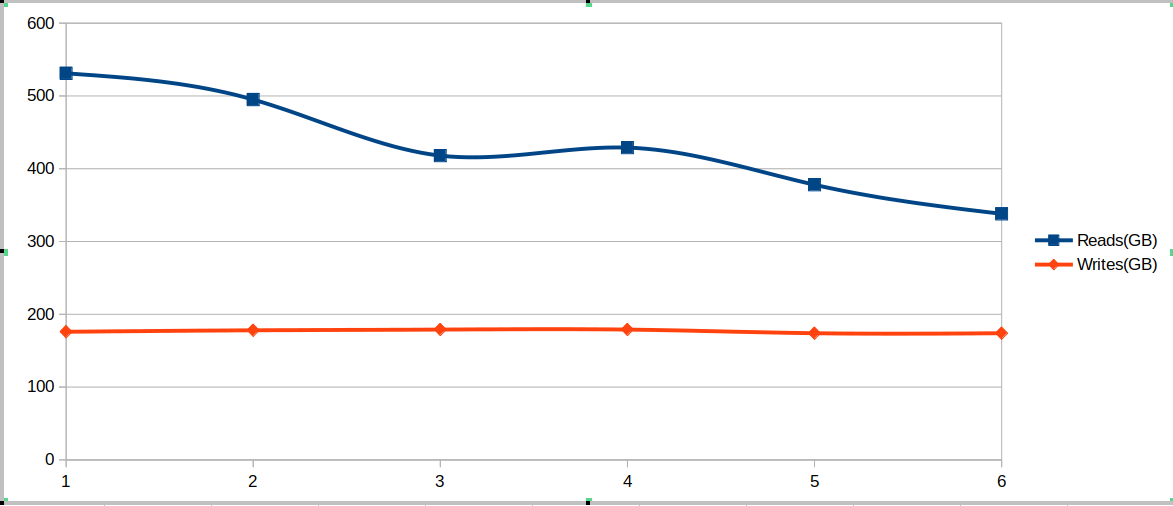
\includegraphics[width=\linewidth]{./fig/rw_pr_pc_th.png}
    \caption{Read-Write traffic over time for PageCache Page Rank
    TeraHeap Spark investigation.}
    \label{fig:rw_pr_pc_th}

    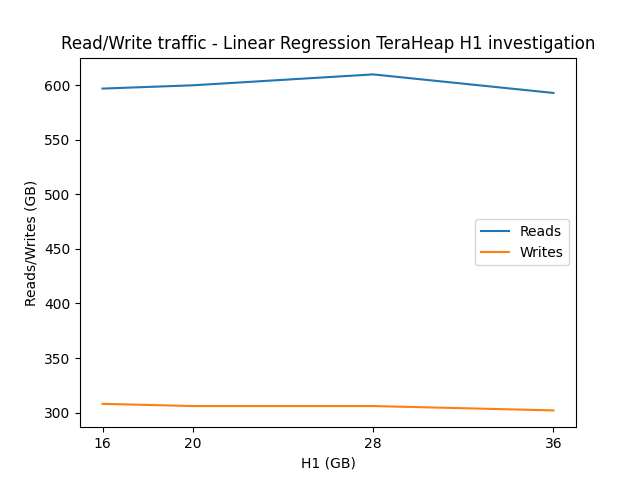
\includegraphics[width=\linewidth]{./fig/rw_linr_h1_th.png}
    \caption{Read-Write traffic over time for H1 Linear Regression
    TeraHeap Spark investigation.}
    \label{fig:rw_linr_h1_th}
\end{figure}

\begin{figure}[thbp]
    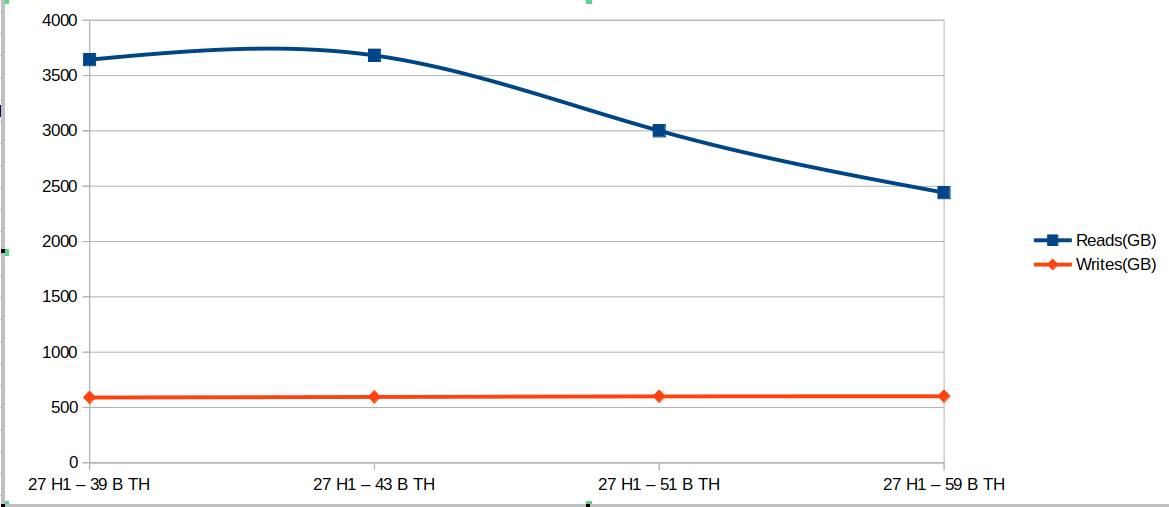
\includegraphics[width=\linewidth]{./fig/rw_linr_pc_th.png}
    \caption{Read-Write traffic over time for PageCache Linear
    Regression TeraHeap Spark investigation.}
    \label{fig:rw_linr_pc_th}

    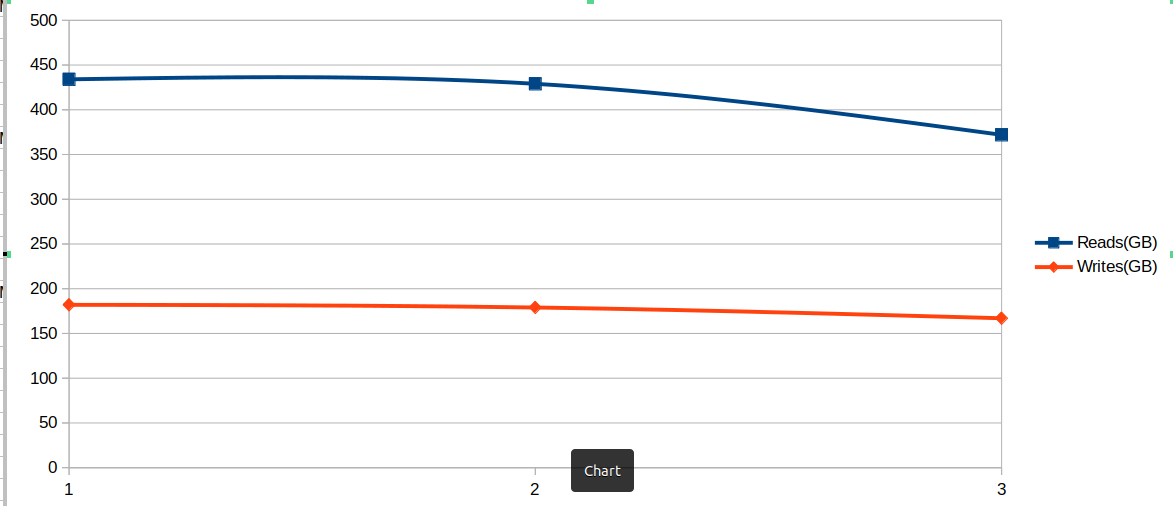
\includegraphics[width=\linewidth]{./fig/rw_pr_h1_th.png}
    \caption{Read-Write traffic over time for H1 Page Rank TeraHeap
    Spark investigation.}
    \label{fig:rw_pr_h1_th}
\end{figure}

\subsection{Java Heap and I/O cache investigation}

Spark's memory management is critical for the performance of big data
analytics applications. In Spark, memory is divided into two
regions: execution memory, and storage memory. Execution memory
is used for storing data during shuffle and join operations and for
caching frequently accessed data. Storage memory is used for storing long lived
cached data. Additionally, Spark uses a combination
of in-memory and disk-based storage to provide efficient data access.
Spark provides various storage levels, including MEMORY-ONLY,
MEMORY-AND-DISK, and DISK-ONLY, to allow users to balance between
memory usage and data availability. We choose MEMORY-AND-DISK for Native Spark 
to cache 50\% of the RDDs in memory and 50\%s off-heap, in the storage device,
to balance memory and storage usage. Spark needs significant amounts
of memory even with the use of an off-heap compute cache. Spark uses
direct I/O to cache RDDs off-heap, while TeraHeap uses MMIO and is in need
of the Linux PageCache. Since our spark applications run within a
memory-limited cgroup in order to assure fair performance in-between
instances, that means that we have to investigate how the different
Spark workloads are performing with different amounts of H1 (Java Heap) for Native-TeraHeap Spark and Giraph and 
and of I/O cache for TeraHeap Spark-Giraph.
Increasing/decreasing H1 automaticaly does the opposite to the I/O
cache, because of the cgroup memory limit. 
Doing this investigation helps us run the colocated experiments using appropriate memory budget
configurations. Moreover we confirm that using a heap amount of 80\% to total DRAM for a group of processes
is the right baseline.
We break the execution time to Major GC, Minor GC and Other time which includes time going to IO from applications threads.

Figure \ref{fig:pr_h1_native} shows performance of single-instance Native Spark
running PageRank with adjustable size for H1 while available DRAM for the rest of the services is kept
steady at 16 GB. This graph shows that decreasing the size of H1
indicates a significant increase to Major GC.
Figure \ref{fig:gcs_pr_h1_native} justifies these claims by showing the obvious
decrease of the number of major gcs.

Figure \ref{fig:pr_h1_th} shows performance of single-instance TeraHeap Spark
running PageRank with adjustable size for H1 while avalaible DRAM for Page Cache is kept
steady at 16 GB. This graph shows that decreasing the size of H1
indicates a significant increase to Minor GC and a slight increase to
Major GC. Figure \ref{fig:gcs_pr_h1_th} justifies these claims by showing the obvious
decrease of the number of minor gcs. 
Figure \ref{fig:pr_pc_th} shows performance of
single-instance TeraHeap Spark running PageRank with adjustable size
for Page Cache while H1 is kept steady at 44 GB. This graph shows that
decreasing the size of PageCache indicates no changes to other time.
Figure \ref{fig:rw_pr_pc_th} justifies these claims by showing read-traffic to be steady.

Figure \ref{fig:linr_h1_native} shows performance of single-instance
Native Spark running LinearRegression with adjustable size for H1
while PageCache is kept steady at 8 GB. This graph shows that
decreasing the size of H1 indicates a significant increase to Major GC
and a slight increase to S/D. Other time remains the same.
Figure \ref{fig:gcs_linr_h1_native} by showing the number of minor-major gcs to decrease
while H1 increases (gc time). 

Figure \ref{fig:linr_h1_th} shows performance of
single-instance TeraHeap Spark running LinearRegression with
adjustable size for H1 while PageCache is kept steady at 8 GB. This
graph shows that decreasing the size of H1 indicates no increase to
GC. Figure \ref{fig:gcs_linr_h1_th} and \ref{fig:rw_linr_h1_th}
justify these numbers by showing the number of major gcs to stay the
same while H1 increases (gc time) and the read-write traffic to remain
steady (other). 
Figure \ref{fig:linr_pc_th} shows performance of
single-instance TeraHeap Spark running LinearRegression with
adjustable size for PageCache while H1 is kept steady at 28 GB. This
graph shows that decreasing the size of PageCache indicates no changes
to Other time. So changes to PageCache do not affect this workload.
Figure \ref{fig:gcs_linr_pc_th} and \ref{fig:rw_linr_pc_th} justify
these numbers by showing the number of minor-major gcs as well as
read-write traffic to remain the same.

\iffalse
\subsection{Metrics} 
When measuring performance, it's
important to choose metrics that provide a comprehensive view of the
system's behavior. In the case of measuring the performance of Spark and Giraph
colocated instances, there are several key metrics that one should consider.
These include heap capacity, which is the amount of memory allocated
GC time is also an
important metric, as it measures the amount of time spent by the JVM
garbage collector in freeing up memory. Serialization/deserialization
time, measured using Java async-profiler \cite{Profiler}, is important for
understanding how much time is spent in this operation, which can be a
bottleneck for some workloads. Other time, which is simply the
difference between total time and GC and serialization/deserialization
time, can provide insight into other factors that may be affecting
performance, but mainly includes the time spent in I/O and also the
time spent by mutator threads to run the application code. Device
traffic, measured using iostat, is important for understanding how
much data is being read from and written to storage devices. CPU idle
and IO wait, measured using mpstat, can help identify how much of the
CPU and I/O resources are being utilized. Finally, average throughput,
measured using Spark Bench, is a good indicator of the overall
performance of the system. Other metrics, such as the total amount of
data processed and the number of minor and major garbage collections,
as measured using jstat, can also provide valuable insights into
system behavior. By considering a range of metrics, one can get a more
accurate and comprehensive view of the performance of Spark instances.

\subsection{Benefits of colocating instances} 
Concurrent execution of workloads provides several benefits.
Firstly, it enables optimal resource utilization by effectively
leveraging the available hardware resources, including CPUs, memory,
and storage. Rather than leaving server resources idle between
workloads, concurrent execution ensures their efficient utilization,
leading to improved throughput and enhanced server efficiency.
Additionally, the consolidation of multiple workloads onto a single
server reduces hardware footprint, simplifies management, and
minimizes operational costs associated with managing multiple servers.

Another advantage is the potential for increased throughput. By
executing multiple workloads concurrently, tasks progress
simultaneously, resulting in faster completion and higher overall
throughput. This approach is particularly valuable when workloads
exhibit varying levels of computational intensity or have different
resource requirements. Concurrent execution allows for efficient
resource allocation, enabling each workload to access the necessary
resources and perform optimally.

Concurrent execution also facilitates workload prioritization,
allowing organizations to allocate resources based on workload
importance or urgency. By running multiple workloads concurrently,
critical or high-priority tasks can be assigned the required resources
and processed in a timely manner. This flexibility in resource
allocation and workload prioritization ensures efficient utilization
of available resources and improves overall performance.

Furthermore, the concurrent execution of workloads supports
experimentation and testing. By running workloads concurrently on the
same server, comparisons, performance benchmarking, and optimization
can be performed in a controlled environment. This concurrent
execution environment enables organizations to evaluate and fine-tune
applications effectively.

Moreover, concurrent execution of workloads allows users to run
workloads along with other users simultaneously. While this is a
method that wouldn't be considered correct in order to evaluate
something because of the interference of other applications running
concurrently, it is something common for the cloud and datacenters
where companies-users share the cloud-server.

Scalability is another advantage of concurrent execution. As data
volumes and processing demands increase, running multiple workloads
concurrently allows for horizontal scalability. Additional 
worker nodes can be added to accommodate larger workloads or handle
additional workloads without the need for significant infrastructure
changes. This scalability ensures that the system can handle growing
demands while maintaining high performance.

In conclusion, the concurrent execution of multiple workloads on
a single server offers significant advantages for performance
optimization. It enables optimal resource utilization, workload
consolidation, improved throughput, workload prioritization,
experimentation, and scalability. By carefully managing resources,
workload scheduling, and monitoring, organizations can achieve higher
performance, reduce infrastructure costs, and simplify management.
\fi

\subsection{Cost estimation}
Renting servers is a common practice for organizations requiring
computational resources, and the question arises as to whether
reducing the monetary cost is possible by achieving higher throughput
and faster workload completion. The relationship between cost
reduction and achieving higher throughput on rented servers is indeed
significant. By optimizing server performance, efficiently utilizing
resources, implementing workload scheduling, and improving
productivity, organizations can realize cost savings. Achieving higher
throughput and faster workload completion can lead to a reduced rental
duration, minimizing the time and associated costs of server usage.
Efficient resource utilization and workload scheduling contribute to
cost reduction by minimizing the number of servers required and
maximizing their utilization. Rental pricing models that take into
account resource utilization or data processed can further reduce
costs for organizations achieving higher throughput. Additionally,
improved productivity resulting from higher throughput and faster
workload completion enhances overall efficiency, allowing
organizations to accomplish more work within the same rental period
and reducing rental expenses. Therefore, pursuing higher throughput
and faster workload completion offers tangible benefits in terms of
monetary cost reduction for organizations renting servers. 

In order to estimate the cost of our evaluation in real-world public clusters we
chose a variety of providers like Amazon \cite{EC2}, Google \cite{GCP} and Microsoft \cite{Azure}. This
way we covered the most known providers and platforms someone would
choose to run their workloads on. We chose 2 machines from each
platform identical to the specifications of our 64, 128 and 256 GB DRAM
machines. These are the cheapest machines of that particular category
offered by the platform. We then used the platform's pricing
calculator to estimate the cost of renting that machine for the time
needed for each configuration to finish execution of all instances. Finally, we noticed that the price for
renting the storage device is really amenable to the cost for renting the machine.
